\documentclass[12pt, a4paper,
 oneside,   
 %%twoside,        
 openright
]{report}

%% Nutné balíčky a nastavení
%%%%%%%%%%%%%%%%%%%%%%%%%%%%

%% Proměnné
\newcommand\city{Pardubice} %% vyplň oficiální název města
\newcommand\district{Pardubický kraj} %% vyplň oficiální název kraje
\newcommand\specialization{Obor č. 18: Informatika} %% -- napiš číslo a název tvého oboru
\newcommand\school{DELTA - Střední škola informatiky a ekonomie, s.r.o.} %% vyplň název školy
\newcommand\consultant{Mgr. Josef Horálek, Ph.D.} %% vyplň jméno svého konzultanta
\newcommand\authorName{Martin Dobruský}  %% vyplň své jméno
\newcommand\publicationYear{2023} %% vyplň rok
\newcommand\mainTitle{Outside The Net} %% vyplň název své práce

\title{\mainTitle} %% -- Název tvé práce
\author{\authorName} %% -- tvé jméno
\date{\publicationYear} %% -- rok, kdy píšeš SOČku

\usepackage[top=2.5cm, bottom=2.5cm, left=3.5cm, right=1.5cm]{geometry} %% nastaví okraje, left -- vnitřní okraj, right -- vnější okraj

\usepackage[czech]{babel} %% balík babel pro sazbu v češtině
\usepackage[utf8]{inputenc} %% balíky pro kódování textu
\usepackage[T1]{fontenc}
\usepackage{cmap} %% balíček zajišťující, že vytvořené PDF bude prohledávatelné a kopírovatelné

\usepackage{graphicx} %% balík pro vkládání obrázků

\usepackage{subcaption} %% balíček pro vkládání podobrázků

\usepackage{hyperref} %% balíček, který v PDF vytváří odkazy

\linespread{1.15} %% řádkování

\usepackage[pagestyles]{titlesec} %% balíček pro úpravu stylu kapitol a sekcí
\titleformat{\chapter}[block]{\scshape\bfseries\LARGE}{\thechapter}{10pt}{\vspace{0pt}}[\vspace{-22pt}]
\titleformat{\section}[block]{\scshape\bfseries\Large}{\thesection}{10pt}{\vspace{0pt}}
\titleformat{\subsection}[block]{\bfseries\large}{\thesubsection}{10pt}{\vspace{0pt}}

\setcounter{secnumdepth}{2}
\setcounter{tocdepth}{1}
\usepackage{fancyhdr}
\pagestyle{fancy}
\renewcommand{\headrulewidth}{1pt}
% mění styl odstavců (odstavec je odsazený o 0.5ex a mezi odstavci je 2ex)
% \setlength{\parindent}{0.5ex}
% \setlength{\parskip}{2ex}

\usepackage{booktabs}

\usepackage{url}

%% Balíčky co se můžou hodit :) 
%%%%%%%%%%%%%%%%%%%%%%%%%%%%%%%

\usepackage{graphicx}
\graphicspath{ {./images/} }

\usepackage{pdfpages} %% Balíček umožňující vkládat stránky z PDF souborů, 

\usepackage{upgreek} %% Balíček pro sazbu stojatých řeckých písmen, třeba u jednotky mikrometr. Například stojaté mí: \upmu, stojaté pí: \uppi

\usepackage{amsmath}    %% Balíčky amsmath a amsfonts 
\usepackage{amsfonts}   %% pro sazbu matematických symbolů
\usepackage{esint}     %% pro sazbu různých integrálů (např \oiint)
\usepackage{mathrsfs}

%% makra pro sazbu matematiky
\newcommand{\dif}{\mathrm{d}} %% makro pro sazbu diferenciálu, místo toho
%% abych musel psát '\mathrm{d}' mi stačí napsat '\dif' což je mnohem 
%% kratší a mohu si tak usnadnit práci

\begin{document}
\pagestyle{empty}
\begin{titlepage}
    \bfseries{ %%% písmo na stránce je tučně
        \begin{center}
            \LARGE{STŘEDOŠKOLSKÁ ODBORNÁ ČINNOST}

            \vspace{14pt}
            \large{ %%%%
                \specialization
            } %%%%

            \vspace{0.4 \textheight}

            \LARGE{ %%%%
                \mainTitle
            }%%%%

            \vspace{0.4\textheight}
        \end{center}
        
        \noindent\Large{\authorName} 

        \noindent\Large{\district \hspace{\stretch{1}}  \city, \publicationYear} 
        
            
    } %%%
\end{titlepage}

\cleardoublepage

%% Úvodní stránka s informacemi
{\bfseries %%% písmo na stránce je tučně
    \begin{center}
        \LARGE{STŘEDOŠKOLSKÁ ODBORNÁ ČINNOST}

        \vspace{14pt}
        {\large %%%%
            \specialization %% -- napiš číslo a název tvého oboru
        } %%%%

        \vspace{0.3 \textheight}

        \LARGE{ %%%%
        \mainTitle
        }

        \LARGE{ %%%%
        Outside The Net
        }%%%%

        \vspace{0.24\textheight}
    \end{center}  
}%%%
{\Large %%%
    \noindent\textbf{Jméno:} \authorName\\
    \textbf{Škola:} \school\\
    \textbf{Kraj:} \district\\
    \textbf{Konzultant:} \consultant\\
} %%%

\noindent \city, \publicationYear

\cleardoublepage

\noindent{\Large{\bfseries{Prohlášení}}}  %% uprav si koncovky podle toho na jaký rod se cítíš, vypadá to pak lépe :) 

\noindent Prohlašuji, že jsem svou práci SOČ vypracoval/a samostatně a použil/a jsem pouze prameny a literaturu uvedené v seznamu bibliografických záznamů.

\noindent Prohlašuji, že tištěná verze a elektronická verze soutěžní práce SOČ jsou shodné. 

\noindent Nemám závažný důvod proti zpřístupňování této práce v souladu se zákonem č. 121/2000 Sb., o právu autorském, o právech souvisejících s právem autorským a o změně některých zákonů (autorský zákon) ve znění pozdějších předpisů. 

\vspace{24 pt}

\noindent V Pardubicích dne 26. března 2023 \dotfill{}\hspace{\stretch{0.5}} 

\hspace{8cm} \authorName

\cleardoublepage

\vspace*{0.8\textheight}
\noindent{\Large{\bfseries{Poděkování}}}

\noindent
Rád bych poděkoval vedoucímu mé práce Mgr. Josefu Horálkovi za cenné rady, věcné připomínky a vstřícnost při konzultacích tvorby tohoto projektu. Dále bych chtěl poděkovat mé rodině a přátelům za jejich podporu v průběhu vývoje.

\cleardoublepage

\noindent{\Large{\bfseries{Abstrakt}}}

\noindent Práce dokumentuje postup vývoje 3D videohry s pracovním názvem Outside The Net. Jedná se o hru přibližující aktuální problematiku kybernetické bezpečnosti. Byla vytvořena v herním enginu Unity za pomocí programovacího jazyku C\#. Cílem projektu/hry je seznámit hráče zábavnou formou s nejčastějšími kybernetickými hrozbami. Modulární architektura umožňuje snadné budoucí rozšíření. Hra je taktéž multiplatformní.

\vspace{18pt}

\noindent{\Large{\bfseries{Klíčová slova}}}

\noindent Programování; Kybernetická bezpečnost; Unity; C\#; Procedurální generace; 3D grafika 

\vspace{18pt}

\noindent{\Large{\bfseries{Abstract}}}

\noindent The thesis documents the development process of a 3D video game with the working title Outside The Net. It is a game presenting current issues of cyber security. It was developed in the Unity game engine using the C\# programming language. The aim of the project/game is to introduce players to the most common cyber threats in an entertaining way. Modular architecture allows for easy future expansion. The game is also multiplatform.

\vspace{18pt}

\noindent{\Large{\bfseries{Keywords}}}

\noindent Programming; Cyber security; Unity; C\#; Procedural generation; 3D graphics

\cleardoublepage

\tableofcontents

\pagenumbering{arabic}
\pagestyle{fancy}
\setcounter{page}{1}

\chapter{Úvod}
\input{Uvod/Uvod.tex}
\input{Uvod/Popis_projektu.tex}

\chapter{Technologie}
\section{Unity}
\label{sec:unity}

Unity je multiplatformní herní engine vyvinutý pro tvorbu videoher a dalších interaktivních aplikací využívajících 2D a 3D grafiku. Engine využívá komponentové architektury a podporuje psaní kódu v programovacím jazyce C\#. \cite{unity}

Engine zjednodušuje proces vývoje her díky používání vizuálních editorů pro tvorbu scén a objektů, kterými lze jednoduše manipulovat pomocí drag-and-drop interakce. Dále obsahuje řadu výkonných nástrojů pro tvorbu fyzikálních simulací, animací, postprocesování obrazu a zvukových efektů. Taktéž obsahuje řadu nástrojů pro tvorbu uživatelského rozhraní a ovládání. Uživatelské rozhraní může také být tvořeno pomocí různorodých komponent, jakož jsou kupříkladu tlačítka, textová pole, posuvníky, checkboxy a další. \cite{unity}

Unity podporuje mnoho platforem jako jsou PC, mobilní zařízení, herní konzole a~VR headsety. Podpora pro tyto platformy zahrnuje jak základní funkce, tak i specifické nástroje a pluginy pro optimalizaci a vývoj pro konkrétní platformy. Unity taktéž podporuje hry multiplayerové a to buď formou vlastních scriptů, nebo předem připravených pluginů. Další výhodou Unity je jeho rozsáhlá komunita, která nabízí mnoho nástrojů, pluginů a~tutoriálů, což umožňuje rychlejší vývoj a snížení nákladů na vývoj hry.

\subsection{Způsob užití v projektu}

Herní engine Unity posloužil pro kompletaci celého projektu.

V první řadě obstaral prostředí pro tvorbu grafického rozhraní, tedy integraci 3D a 2D herních komponent. Zároveň také tvorbu uživatelského rozhraní a ovládání. Ovládání bylo zprostředkováno formou vstupních inputů. Uživatelské rozhraní bylo tvořeno v enginu za pomocí komponentu Canvas a to rastrovou i vektorovou grafikou. Pro texty byl využit aktualizovaný textový systém. Původní nejpoužívanější variantou byly základní textové komponenty, nyní došlo k přechodu na TMP (TextMeshPro) komponenty, které se mimo jiné starají o výpisy textových polí \cite{unity_tmp}.

Další funkcí tohoto nástroje, která byla využita, je práce se světlem a zvuky. Unity v~základu nabízí velice jednoduchou práci s těmito prosředky. I v případě, že vývojář vyžaduje komplexnější zásahy do fungování těchto prostředků, je možné toto učinit v~nastavení jednolivých komponent nebo build nastavení hry.

V neposlední řadě také enigne zajistil samotný export spustitelného programu pro různé operační systémy i s podporou nejnovějšího proprietárního herního middlewaru \cite{unity_api}.

\subsection{Alternativní herní enginy}

Alternativ k hernímu enginu Unity je více a každá přináší různé výhody a nevýhody. V~této práci budou představeny tři z nejznámějších alternativ k Unity.

První alternativa je Unreal Engine, který je vytvořen společností Epic Games. Unreal Engine poskytuje široké spektrum funkcí pro tvorbu 3D her a virtuální reality. Jeho hlavní předností je vysoká kvalita grafiky a pokročilé možnosti simulace fyziky. Unreal Engine je také vhodný pro vytváření her s velkým rozsahem a detaily. Nevýhodou je vyšší náročnost na hardwarové a softwarové prostředky. \cite{unreal_engine}

Unreal Engine nebyl zvolen z důvodů vyšší komplexnosti, než je k tvorbě projektu zapotřebí. Jak bylo zmíněno výše, Unreal Engine je vhodný pro vytváření her s velkým rozsahem a detaily. Vzhledem k tomu, že projekt je zaměřen na vytvoření jednoduché hry s nízko-polygonovou grafikou, byla zvolena alternativa Unity.

Druhá alternativa je CryEngine, který je vytvořen společností Crytek. CryEngine je podobně jako Unreal Engine zaměřen na tvorbu 3D her s vysokou kvalitou grafiky a pokročilými funkcemi simulace fyziky. Hlavní výhodou CryEngine je jeho rychlost a efektivita, která umožňuje vývojářům snadno vytvářet velké a rozsáhlé světy. Nevýhodou CryEngine je vysoká cena a náročná úprava. \cite{cryengine}

CryEngine nebyl taktéž zvolen z důvodů vyšší komplexnosti, než je k tvorbě projektu zapotřebí. Jak bylo zmíněno výše, tak i CryEngine je spíše vhodný pro vytváření her s~velkým rozsahem a detaily. 

Třetí alternativa je Godot Engine, který je open-source herní engine vyvíjený komunitou. Godot Engine poskytuje snadné použití a rychlou návratnost při tvorbě 2D a 3D her. Hlavní výhodou Godot Engine je jeho flexibilita a možnost použití na různých platformách. Godot Engine je také zdarma a nevyžaduje žádné licenční poplatky. Nevýhodou je menší komunita a menší podpora než u Unity, Unreal Engine nebo CryEngine. \cite{godot}

Herní engine Godot byl druhou nejvíce vhodnou variantou pro tvorbu projektu takovéhoto typu. Ve výsledku bylo zvoleno Unity z důvodu osobních preferencí a zkušeností.
\\\\
\section{JetBrains Rider}

JetBrains Rider je IDE speciálně navržené pro vývoj aplikací v jazyce C\# a .NET. Jedná se o multiplatformní IDE, které je k dispozici pro všechny nejběžnější operační systémy.
Rider nabízí širokou škálu funkcí, včetně funkce refaktorování, inteligentního dokončování kódu, ladění aplikací a integrace s nástroji jako je Git. \cite{rider}

Rider také poskytuje podporu pro různé typy projektů, včetně projektů pro ASP.NET, Unity, Xamarin a .NET Core. IDE je také kompatibilní s různými databázovými systémy, jako jsou Microsoft SQL Server, MySQL a PostgreSQL.
V Rideru jsou také k dispozici nástroje pro testování kódu a prohlížení výsledků testování.

\subsection{Způsob užití v projektu}

Při vývoji bylo IDE Rider propojeno s herním enginem Unity. Posloužilo pro psaní veškerého kódu projektu.

Toto IDE bylo pro práci zvoleno z důvodu vysoké integrace s herním engine Unity. Příkladem by mohly být ukazatele odkazování metod na vnější objekty v enginu. Díky tomu lze jednodušeji optimalizovat a refaktorovat kód. K optimalizaci kódu taktéž přispívá doporučení pro privatizaci veřejných proměnných, které by mohly být privátními.

Rider má taktéž plugin pro Unity s názvem RiderFlow \cite{riderflow}. Plugin umožňuje ladit aplikaci přímo v Unity editoru, což je užitečnou funkcí při ladění chyb v herním engine. Bohužel nebylo možné tento plugin využít, protože v momentální verzi je plugin velmi nestabilní a nespolehlivý.

\section{Blender}

Blender je open-source 3D modelovací nástroj, který nabízí vývojářům a umělcům širokou škálu funkcí pro tvorbu 3D modelů, animací, vizualizací a interaktivních aplikací.

Jedná se o výkonný nástroj, který umožňuje vytvářet vysoko kvalitní 3D modely pomocí různých technik, včetně polygonálních modelů, NURBS, sculptingu a dalších. Vývojáři mohou také vytvářet animace pomocí keyframe animace, simulací fyziky, ragdoll animace a dalších technik.

Blender poskytuje řadu nástrojů pro tvorbu textur a materiálů, včetně podpory pro PBR materiály, texturování procedurálními mapami a dalšími technikami. Vývojáři také mohou využívat různé osvětlovací techniky, včetně výpočtu globálního osvětlení (GI), ray tracingu a dalších. \cite{blender}

Také umožňuje vývojářům používat různé pluginy a rozšíření funkčnosti nástroje. Blender má také rozsáhlou komunitu, která nabízí různé nástroje, šablony a tutoriály pro vývojáře.
\\\\
\subsection{Způsob užití v projektu}

Software Blender byl využit pro tvorbu některé 3D grafiky. Původním plánem bylo realizovat veškerou 3D grafiku samostatně. Již v rané fázi projektu bylo zřejmé, že komplexní tvorba veškeré grafiky by měla za následek výrazné zpomalení vývoje a tedy i fakt, že by se některé funkce do alfa verze vůbec nedostaly. Z tohoto důvodu byl pro většinu grafiky využit asset pack zaměřený na low-poly kancelářské modely \cite{unity_asset}.

\chapter{Realizace}
\section{Struktura projektu}

\begin{figure}[ht]
    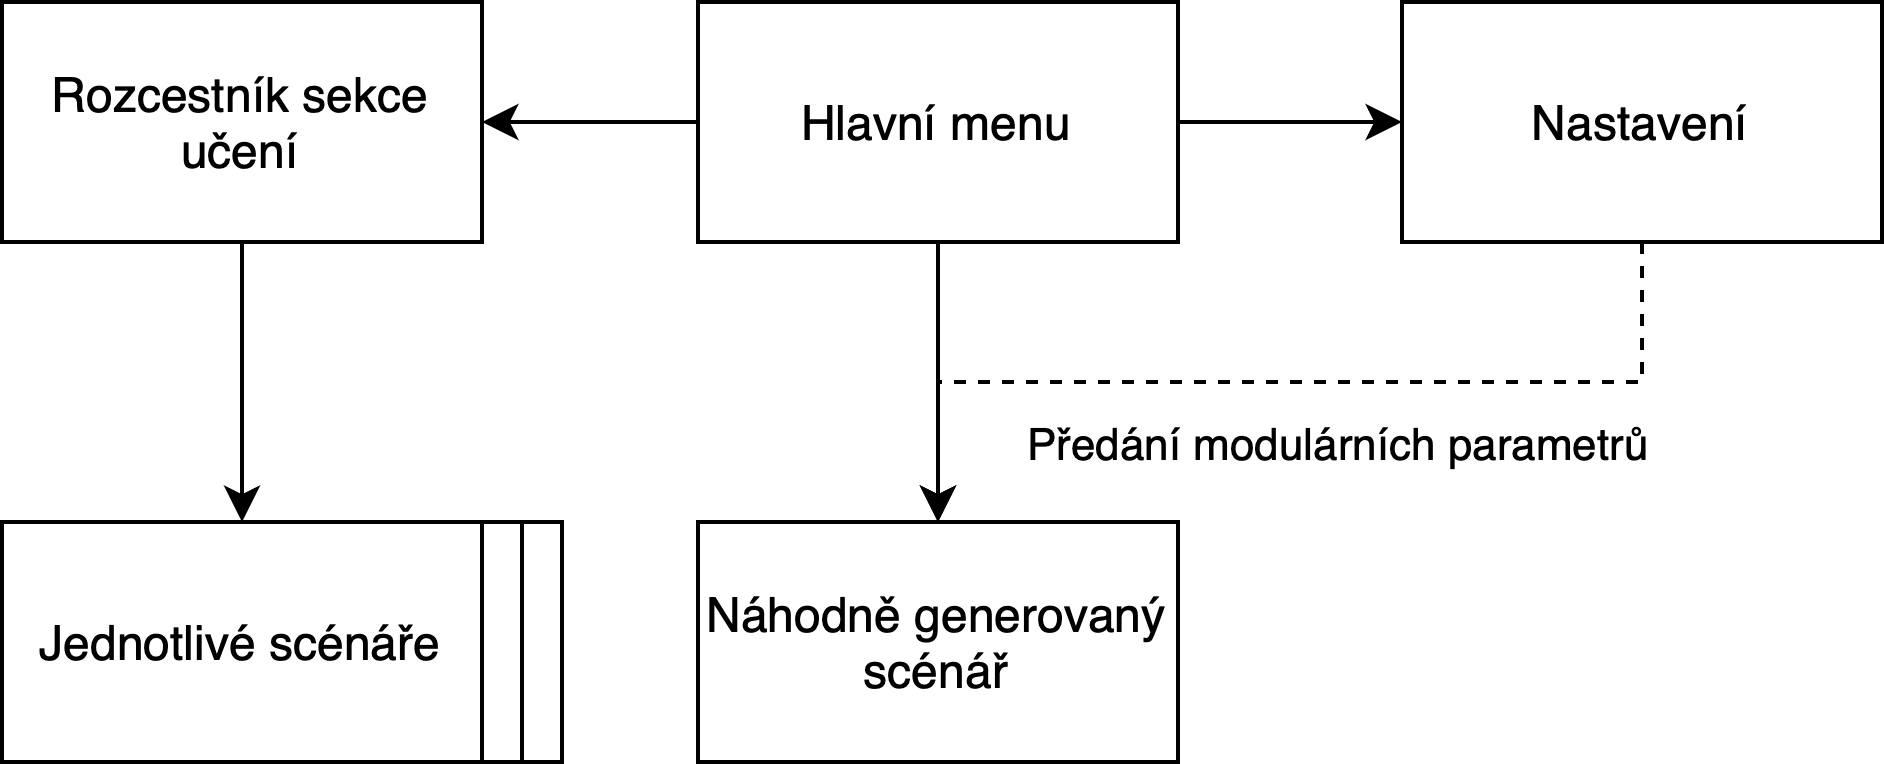
\includegraphics[width=\columnwidth]{struktura_projektu.png}
    \centering
    \caption{Struktura návaznosti scén projektu}
    \label{fig:struktura_svg}
\end{figure}
\subsection{Menu}
Projekt je rozdělen do tří scén.

První z nich je úvodní obrazovka – dále zvaná menu. Menu obsahuje tři obrazovky, které jsou propojeny spojitou animací kamery. Hlavní z těchto obrazovek se zobrazí hráči po spuštění hry. Slouží jako hlavní rozcestník do dalších částí projektu a to za pomocí čtyř tlačítek: Start random scenario, Start learning, Settings a Quit. Tato dvojrozměrná interaktivní grafika je integrována do trojrozměrného prostoru. Každý z přechodů do jiné scény je tvořen plynulým přechodem přes černou barvu. Tyto přechody neslouží pouze v estetické rovině, ale zároveň zajišťují čas dostatečný pro načtení veškerých objektů, scriptů a světelných map a jiných prvků renderovaných v ostatních scénách bez použití načítacích obrazovek. Grafické vyzobrazení scény je viditelné na obrázku \ref{fig:menu_img}.

Druhá z obrazovek slouží jako rozcestník pro výukové sekce. Obsahuje několik interaktivních tlačítek odkazujících do výukových scénářů. Tato grafika je taktéž začleněna do trojrozměrného prostředí.

Poslední obrazovka je obrazovka nastavení. Blíže je popsána v kapitole \ref{sec:nastaveni}.
\\


\begin{figure}[ht]
    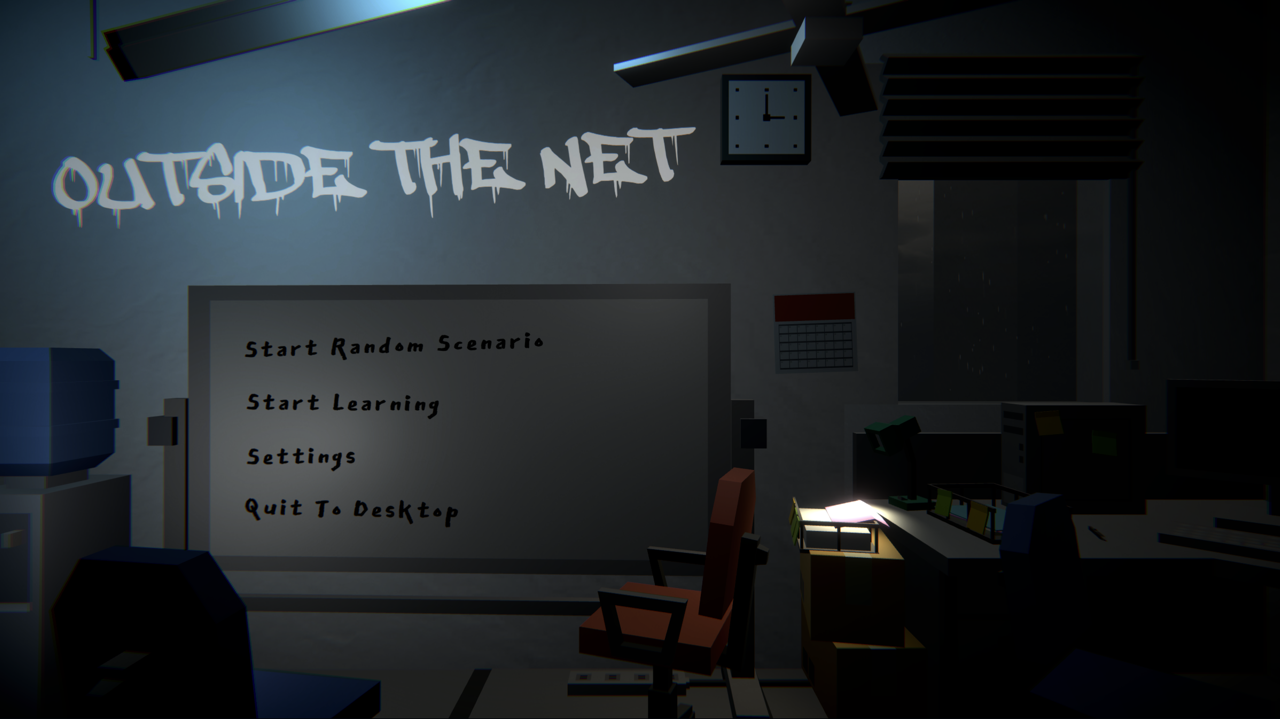
\includegraphics[width=\columnwidth]{menu.png}
    \centering
    \caption{Ukázka grafického vzhledu úvodní obrazovky hry}
    \label{fig:menu_img}
\end{figure}
\subsection{Nastavení}
\label{sec:nastaveni}
Poslední obrazovkou je obrazovka nastavení. Tato obrazovka je stejně jako všechny ostatní integrována do úvodní scény a je zobrazena po animaci přechodu kamery. Obsahuje několik nastavení, která jsou přímo propisována do zbytku hry a ovlivňují vstupní parametry v~náhodném herním scénáři.

První z nastavení je zobrazení FPS. Tento ukazatel je vypočítáván přímo ve hře v~závislosti na opravdovém času vykreslování. Slouží hráči k lepší orientaci týkající se výkonu hry a může pomoci při výběru vhodných grafických nastavení.

Druhým nastavením je nastavení obtížnosti hry, toto nastavení se projevuje při generaci mapy i při následném průběhu hry. Čím těžší je obtížnost, tím více počítačových stanic mapa obsahuje. Následně jsou během hry přidělovány hrozby v intervalu odpovídajícím obtížnosti hry. Těžší nastavení opět odpovídá větší intenzitě zobrazovaných problémů.

Dalším nastavením je celková hlasitost hry. Toto nastavení ovlivňuje celkovou hlasitost hry, včetně hudby a zvuků. Interaktivní posuvník označený popiskem Master Volume vyjadřuje porcentuální hlasitost vůči nejvyšší hlasitosti OS.

V neposlední řadě je několik nastavení věnováno grafickému zobrazení. Tato nastavení mají za úkol zajistit správné zobrazení a co nejplynulejší běh hry. Rozlišení mění rozlišení obrazu v pixelech. Grafická nastavení jsou zaobalena do přehledných nabídek v rozbalovacím okně. Na pozadí dochází k výměně Universal Renering Pipeline objektů v nastavení URP. Tyto objekty mění například rozlišení textur, chovaní a kvalitu stínů nebo zobrazení a intenzitu postprocessingu. Všechny tyto nastavení jsou výchozí a jsou přepsány při spuštění hry podle posledních vybraných nastavení.
\begin{figure}[ht]
    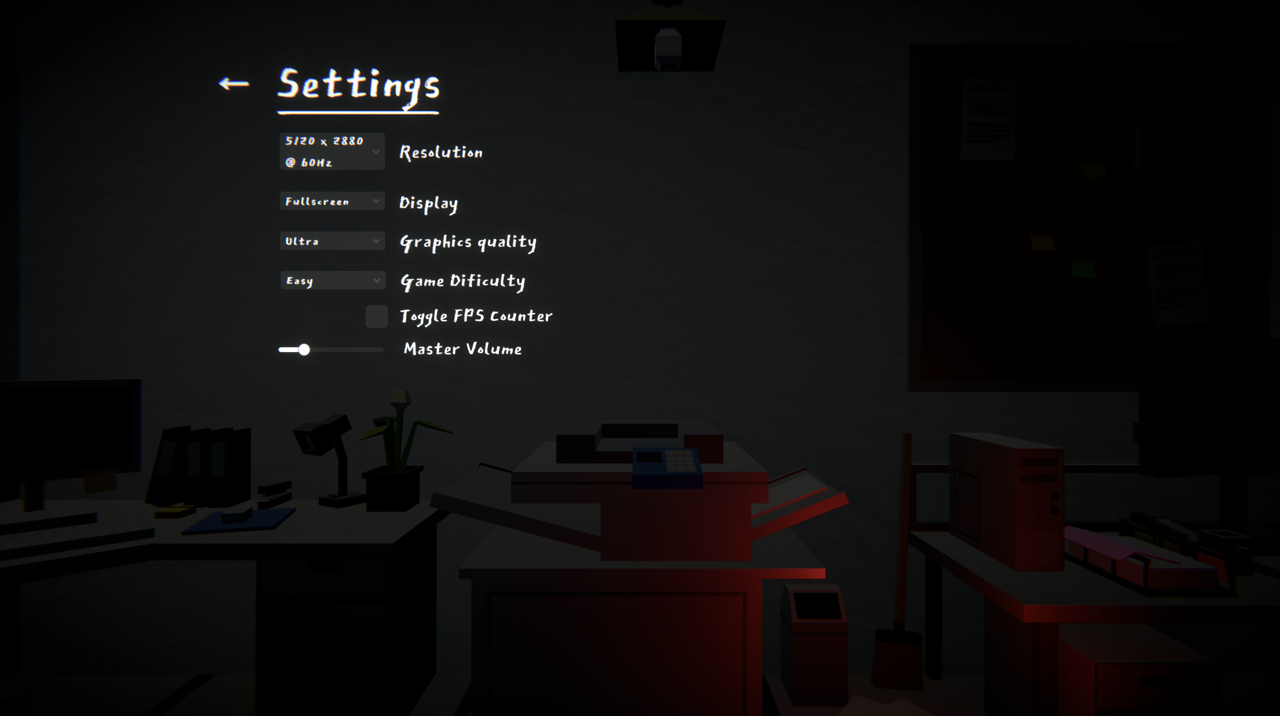
\includegraphics[width=\columnwidth]{nastaveni.png}
    \centering
    \caption{Obrazovka herních nastavení}
    \label{fig:nastaveni_img}
\end{figure}
\subsection{Rozdělení na hratelné sekce}
\label{sec:rozdeleni_sekci}

Hra je rozdělena na dvě hratelné sekce.

Tyto sekce mají odlišný účel a jsou samostatně spustitelné z hlavní nabídky. Jsou tvořeny dvěma na sobě nezávislými scénami. Sekce Náhodně generovaného scénáře (Start Random Scenario) byla zamýšlena jako primární herní součást, protože nabízí kombinaci všech vytvořených mechanik i vybraných implementovaných hrozeb. Druhou sekcí je sekce Učení (Learning), která zastává nenahraditelnou funkci seznámení hráče s implementovanými mechanismy a zároveň i s ovládáním a fungováním hry samotné.
\subsubsection{Sekce náhodně generovaného scénáře}
\label{sec:nahodny_scenar}

Sekce náhodně generovaného scénáře je první a primární herní sekcí.

Po spuštění je hráč přenesen na herní mapu. Herní mapa je tvořena jednopodlažním kancelářským komplexem. Tato mapa je vygenerována za pomocí algoritmu náhodného rozmístění objektů, blíže popsaného v kapitole \ref{sec:finalni_provedeni_mapy}. Tato generace slouží k umožnění repetitivního hraní tohoto scénáře. Vzniká tak pro hráče možnost čelit modifikovaným rozložením a tehdy i možnost své znalosti ověřit a zdokonalit opakovaným hraním. Zároveň také tento fakt přispívá k zábavnosti celého herního módu.

Hráčova kamera zabírá pohled shora na tento komplex. Hráč má možnost volného pohybu nad celým komplexem a zároveň otáčení pohledu kamery dle libosti. Kamera se dá teké přiblížit a oddálit.

Po mapě jsou rozmístěny počítačové stanice. Hráč má možnost s těmito stanicemi interagovat stisknutím levého tlačítka myši. Po stisknutí tlačítka je otevřeno počítačové rozhraní. Toto rozhraní je taktéž náhodně generováno, pro dokreslení již zmiňovaného efektu. Tento proces je více popsán v kapitole \ref{sec:generace_rozhrani}. Rozhraní obsahuje všechny očekávané prvky včetně pozadí, souborů a hlavní lišty.

Posledním hlavním prvkem je simulovaný příkazový řádek. Tento příkazový řádek imituje funkcionality několika nejběžnějších příkazů. Hráč se tedy s těmito příkazy seznámí a následně je využije při řešení problematiky hrozeb.
\subsubsection{Sekce výuky hráče}
\label{sec:vyuka_scenar}

Sekce výuky hráče je druhou hratelnou sekcí.

První scénář v této sekci je věnován seznámení hráče s ovládáním, fungováním a průběhem celé hry a jejích jednotlivých hratelných sekcí. Tento scénář je tvořen jednoduchou scénou s piktogramy znázorňujícími ovládací prvky. Scénář je stavěn způsobem, aby hráč musel využít veškeré ovládací prvky k jeho dokončení. Každé úspěšné splnění zadání je znázorněno barevným indikátorem a přesunem k dalšímu z úkolů.

Další scénáře jsou věnovány jednotlivým integrovaným hrozbám, v aktuální verzi jsou to: Malware a Ransomware.

Dále bylo vytvořeno několik scénářů, které jsou primárně textové a jmenované hrozby nejsou začleněny do hlavní sekce hry. Jedná se o scénáře, které jsou zaměřeny na problematiku bezpečnosti osobních údajů a jejich ochranu. Tyto prvky problematiky nebyly do náhodně generovaného herního módu začleněny především z důvodu jejich povahy. Jsou kritické, ale jejich začlenění do hry by nebylo zábavné. Přesto jsou tyto prvky zahrnuty v~sekci výuky hráče, jelikož jsou asi nejčastěji vyskytujícími se problémy. Patří mezi ně problematika hesel, phising se zaměřením na e-mailovou komunikaci a uchovávání osobních dat.

Scéna vždy obsahuje textového průvodce, který touto formou popíše dané téma a~následně vyzve hráče k vyzkoušení praktické ukázky. Ukázka jedné ze scén je viditelná na obrázku \ref{fig:uceni0_img}.

\begin{figure}[ht]
    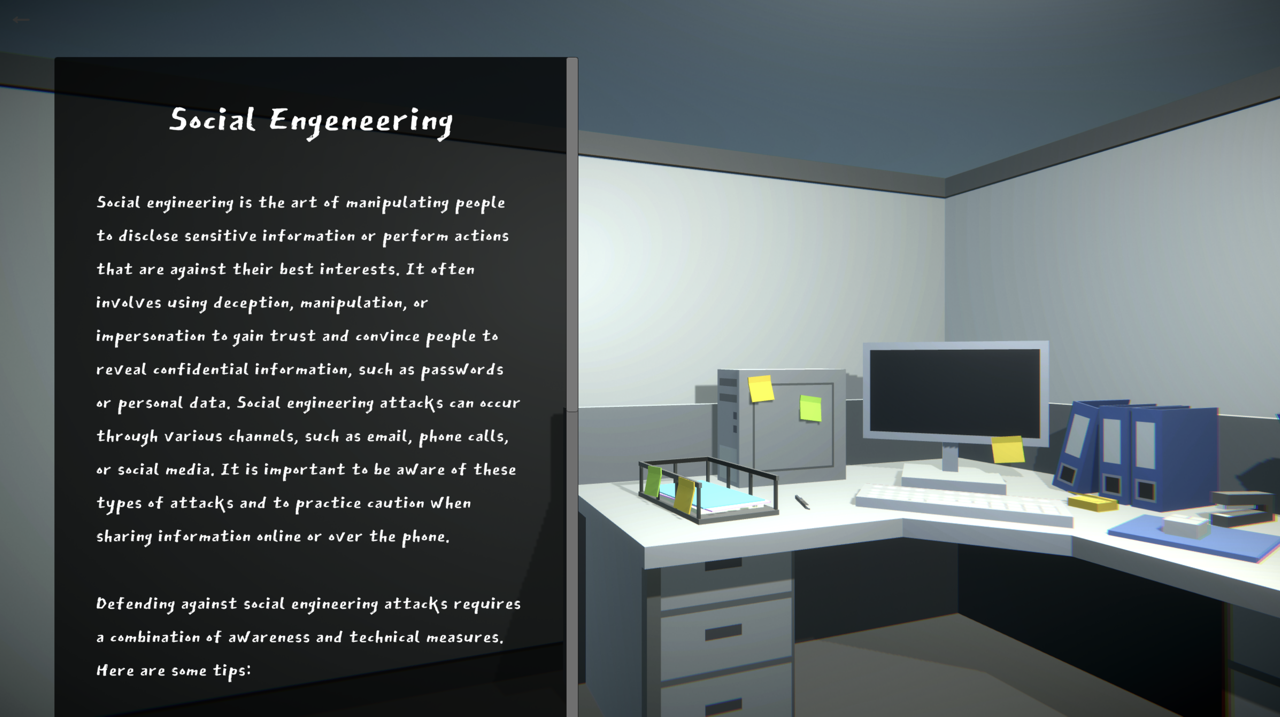
\includegraphics[width=\columnwidth]{uceni0.png}
    \centering
    \caption{Ukázka grafického vzhledu obrazovky s výukovým scénářem}
    \label{fig:uceni0_img}
\end{figure}


\section{Integrované kybernetické hrozby}
Do hry je integrováno několik kybernetických hrozeb. Při výběru byly zohledněny nejaktuálnější hrozby dle několika ověřených zdrojů. Jedním z nich je průzkum společnosti ENISA pro rok 2022. \cite{enisa}
\subsection{Malware}

První z integrovaných hrozeb je nejčastější hrozbou dnešní doby.

Malware je zkratka pro "malicious software", což v překladu znamená "škodlivý software". Jedná se o jakýkoli typ softwaru, který byl navržen tak, aby způsobil škodu na počítači, síti nebo na datech, která jsou na těchto systémech uložena.

Existuje mnoho druhů malware, včetně virů, trojanů, spyware, adware, ransomware a~dalších. Tyto programy se mohou šířit různými způsoby, například pomocí emailových příloh, souborů ke stažení z internetu, infikovaných webových stránek nebo pomocí externích paměťových zařízení.

Malware může mít různé cíle, včetně krádeže osobních údajů, poškození systému, šíření spamu, zobrazování reklam nebo blokování přístupu k datům a požadování výkupného. Může také být použit k infikování dalších počítačů v síti nebo k vytvoření botnetu, což je síť počítačů infikovaných malwarem, která může být ovládána z jednoho centrálního místa.

Ochrana proti malware zahrnuje instalaci antivirového software, aktualizace operačního systému a aplikací, používání silných hesel a opatrnost při otevírání neznámých souborů nebo klikání na neznámé odkazy.

Více detailních inforamcí je obsaženo v knize Thread Landsacpe 2022 na stranách 49 až 53. \cite{enisa}
\subsection{Ransomware}

Ransomware je škodlivý software, který blokuje přístup k počítačovému systému nebo šifruje data a vyžaduje výkupné za jejich obnovení. Tento typ útoku je obvykle spuštěn kliknutím na odkaz nebo stažením souboru z podezřelého zdroje. Jakmile se ransomware dostane do počítačového systému, začne šifrovat data a zobrazuje výzvu k platbě výkupného za obnovení dat. Útočník obvykle požaduje platbu v kryptoměně, aby bylo obtížnější jeho vystopování.

Ransomware se může šířit prostřednictvím e-mailových příloh, škodlivých reklam nebo prostřednictvím nezabezpečených sítí. Ochrana proti ransomware zahrnuje pravidelné zálohování dat, instalaci aktualizací softwaru a firewally, používání silných hesel a pozornost při stahování souborů a klikání na odkazy z neznámých zdrojů.

Pokud se stane, že váš počítač je napaden ransomware, nedoporučuje se platit výkupné, protože to nezaručuje, že získáte svá data zpět a může motivovat útočníky k dalšímu útoku.

Více detailních inforamcí je obsaženo v knize Thread Landsacpe 2022 na stranách 43 až 48. \cite{enisa}
\subsection{Phishing}

Phishing je forma útoku, při které se útočník snaží získat citlivé informace od oběti prostřednictvím falešné identity a sociálního inženýrství.

To může být dosaženo pomocí falešných emailů, textových zpráv nebo webových stránek, které vypadají jako legitimní zdroje. Útočník využívá důvěryhodnosti a nevědomosti oběti a získané informace mohou být použity k výrazným finančním škodám.

Ochrana proti phishingu zahrnuje opatrnost při klikání na odkazy a zadávání citlivých informací, používání silných hesel, aktualizaci antivirového software a firewally a~pravidelné školení zaměstnanců ohledně této formy útoku.

Více detailních inforamcí je obsaženo v knize Thread Landsacpe 2022 na stranách 54 až 62. \cite{enisa}

\section[Řešení generovaného scénáře]{Technické řešení generovaného scénáře}
\subsection{Procedurální generace mapy}

\subsubsection{Prvotní pokus s generací za pomocí šachovnicového paternu}
Prvotním pokusem bylo vytvoření mapy za pomoci systému umísťování předem vytvořených prefabů v šachovnicovém paternu. Tento systém se dá kupříkladu velice efektině využít ve tvorbě některých 2D map. V tomto případě systém sice fungoval, ale byl velice omezený. Mapa působila nesoudržně a nebyla píliš přehledná. Z tohoto důvodu byl tento systém nahrazen a začala práce na mnohem komplexnějším systému, který na teoretické rovině nabízel mnoho výhod a velikou flexibilitu. Velmi raná verze mapy vytvořená pomocí šachovnicového systému je na obrázku \ref{fig:mapa_sachovnice}. Nový systém generace je popsán v kapitole níž v sekci \ref{sec:proceduralni_generace_mapy}.

\begin{figure}[ht]
    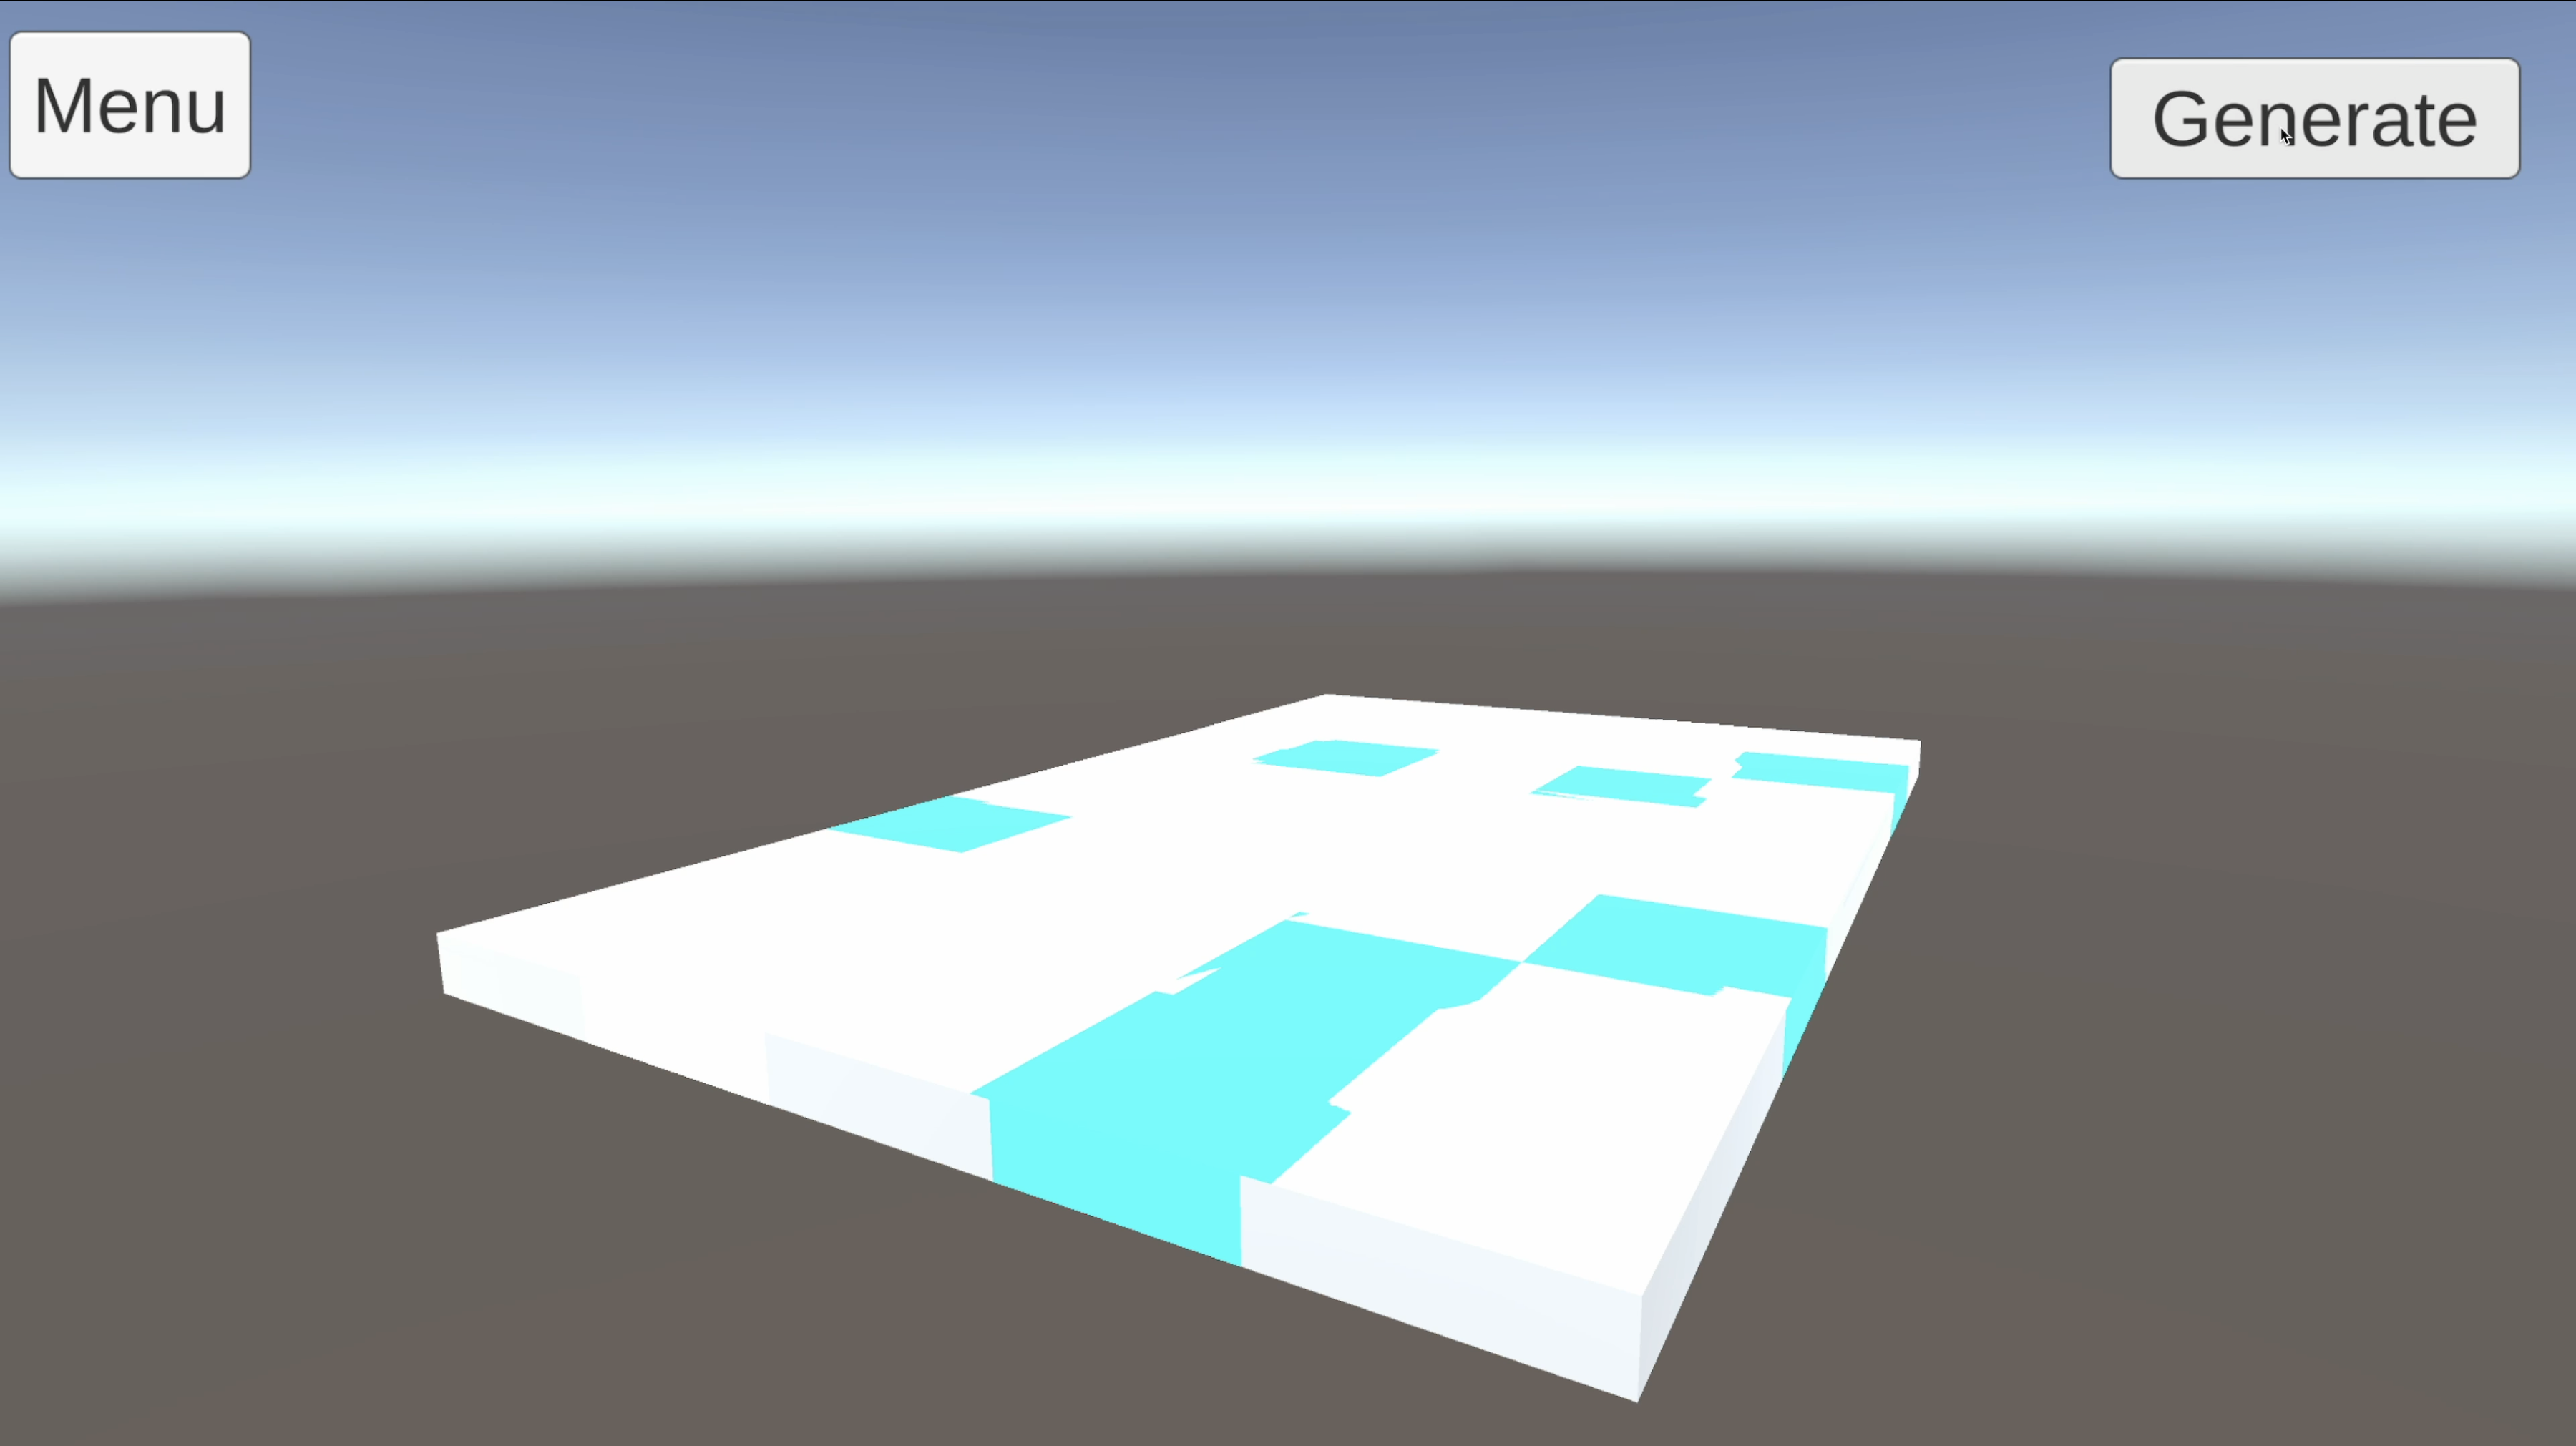
\includegraphics[width=\columnwidth]{mapa_sachovnice.png}
    \centering
    \caption{Raná verze mapy vytvořená pomocí šachovnicového systému}
    \label{fig:mapa_sachovnice}
\end{figure}

\subsubsection{Procedurální generace s náhodnými parametry}
\label{sec:proceduralni_generace_mapy}

Druhým pokusem bylo vytvoření mapy za pomoci procedurální generace s náhodnými parametry. Tento systém by nabízel velkou flexibilitu a mnoho možností.

Systém fungoval na principu náhodného výběru vstupních parametrů v limitních mezích. Tyto parametry rozhodly o velikosti první z místností. Následně byly vytvořeny další místnosti, které byly umístěny v okolí první místnosti tak, aby na ni přímo navazovaly, ale nepřekrývaly ji. Bylo zapotřebí využít délky a šířky první místnosti, vygenerovat délku a šířku místnosti druhé a v závisloti na hodnotách posunout pivotní bod základny druhé místosti na správné místo v 3D prostoru tak, aby místnosti navazovaly. Následně byla vygenerována další místnost a tak dále.

Poté došlo k vytvoření stěn o pevně dané šířce na hranách podstav místností. Délky těchto stěn přímo odpovídaly délkám a šířkám místností. Střed stěny byl umístěn v polovině délky podstavy od středu v odpovídající výšce.

Dalším prvkem bylo určení druhu místnosti. Bylo vytvořeno několik kategorií místností: kancelář, místnost nadřízeného, konferenční místnost, chodba, odpočívárna a sklad. Tyto kategorie byly následně přiděleny každé místnosti v závislosti na jejích parametrech. Podmínkou bylo, že některé místosti musí být obsaženy z důvodu průběhu hry. Pokud by kupříkladu nebyla přítomna kancelář, tak by chyběly potřebné počítačové stanice. Dalším příkladem je místnost nadřízeného, která musí obsahovat počítačovou stanici. Proto byly tyto kritické kategorie přiděleny v úvodu a to největší a nejmenší z místností. Dále byly zohledněny rozměry místností a jejich pozice na mapě. Například pokud byla místnost podlouhlá, tak se jednalo o chodbu. Zbytek místností byl přiřazen ze zbytku kategorií náhodně.

Tento systém byl velmi flexibilní a nabízel velké množství možností. Bohužel se nepodařilo jeho dokončení. Problém nastal při umísťování prefabů v prostoru. K umístění došlo, ale postup byl neefektivní a výsledek byl nesystematický. Proto byl tento systém nahrazen za systém, který je popsán v následující kapitole. Stále ale věřím, že se jedná o nejvíce zajímavý a flexibilní systém, u kterého není možné vyloučit jeho použití v budoucnu.

\subsubsection{Finální provedení}
\label{sec:finalni_provedeni_mapy}

Výsledné řešení je ve svém provedení částečně jednodušší než řešení popsané v předchozí kapitole. Výsledek je však dostatčný pro tvorbu iluze mnoha kombinací a opakujícího se prostředí mapy.

Generace funguje na principu umísťování prefabů do náhodných pozic z předem známého pole bodů v trojrozměrném prostoru. Mapa je prakticky statická a dochází tedy převážně ke změně pozic prefabů.

V prvním kroku je definováno pole pozic, které obsahuje několik možných pozic, na kterých lze umístit objekty. Poté je vytvořena funkce, která náhodně vybírá několik pozic z pole a na tyto pozice umísťuje náhodně vybrané objekty. Pro každý typ objektu je tento proces samostaný a proběhne tedy několikrát.

V kroku druhém jsou na mapy doplněny dodatečné objekty v závislosti na zabraných pozicích.

Tento systém je v dosavadní alfa verzi dostačující, ale jak již bylo zmíněno výše, je možné v budoucnu obnovit původní myšlenku procedurální generace, která by umožnila vytvořit více možností a vytvořit tak více dynamické prostředí.

\begin{figure}[ht]
    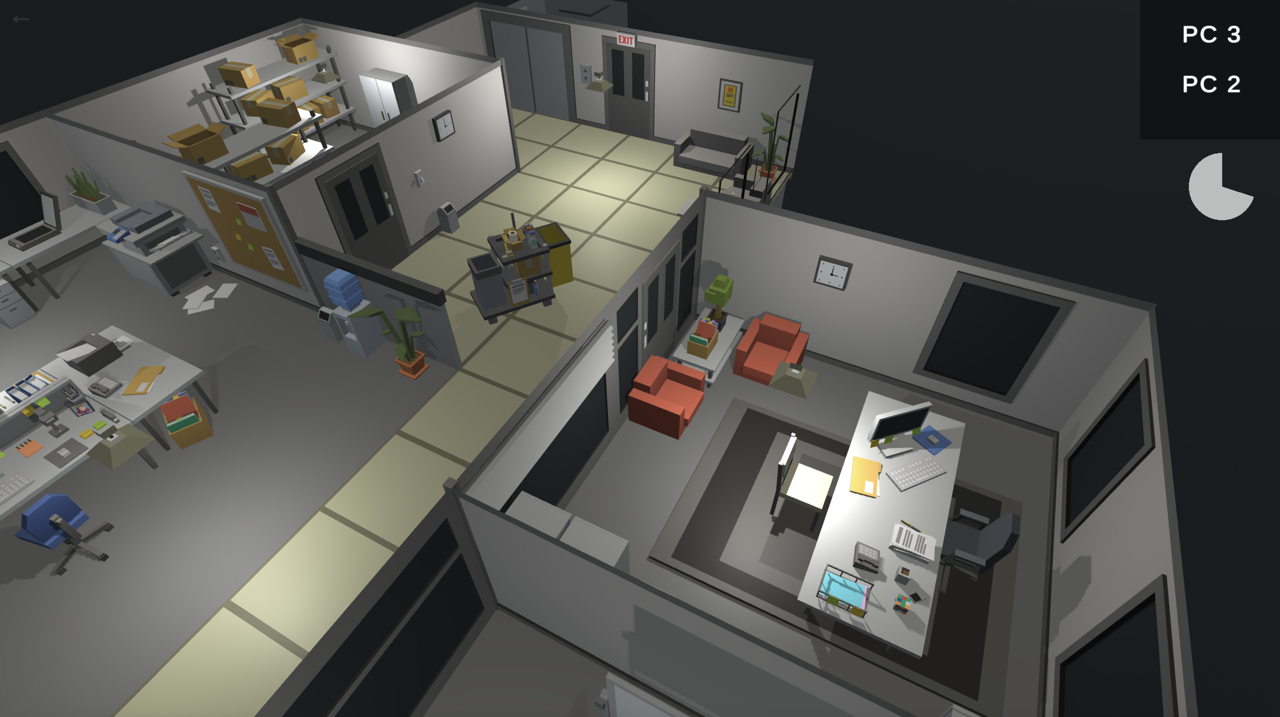
\includegraphics[width=\columnwidth]{mapa0.png}
    \centering
    \caption{Herní mapa kancelářského komplexu}
    \label{fig:mapa0_img}
\end{figure}

\subsection{Procedurální generace počítačového rozhraní}
\label{sec:generace_rozhrani}

Po výše zmíněné generaci mapy je třeba umístit na mapu jednotlivé počítače. Je tak učiněno opět za pomocí několika možných pozic umístění. Každý počítač je identifikován fiktivním jménem jeho vlastníka. Toto jméno je generováno z předvytvořeného pole. Po umístění PC na mapu je generováno počítačové rozhraní.

Počítačové rozhraní je pro každý počítač na mapě generováno unikátně. Rozhraní je inspirováno Linuxovým rozhraním.

Na levé straně simulovaného počítačového rozhraní se nacházejí soubory, jejichž jména, ikony a koncovky jsou náhodně generovány.

Původně byly soubory náhodně rozmístěny po celé ploše. Tento přístup byl však matoucí a ani příliš neodpovídal situacím z reálného světa. Je sice pravdou, že systémy jako je MacOS umožňují umísťovat soubory libovolně po celé ploše, většinou však uživatelé stejně dodržují určitou systematičnost v jejich rozmístění. Proto bylo rozhodnuto, že soubory budou rozmístěny do sloupců na levé části obrazovky.

Prvním krokem generace je výběr aktuálního sloupce. Na začátku se tedy jedná o~sloupec s indexem nula. Následně je vybrán náhodný počet souborů, které budou v sloupci vytvořeny.

V dalším kroku je vybrána textura souboru z již existujících textur. Odpovídající textuře je přiřazen název z existujícího pole názvů a odpovídající přípona. Jedním z~prvků je taktéž možnost, že je soubor škodlivý. To lze poznat podle podezřelého názvu nebo přípony. V takovém případě je úkolem uživatele soubor smazat.

Tento proces je opakován v každém ze sloupců.

\begin{figure}[ht]
    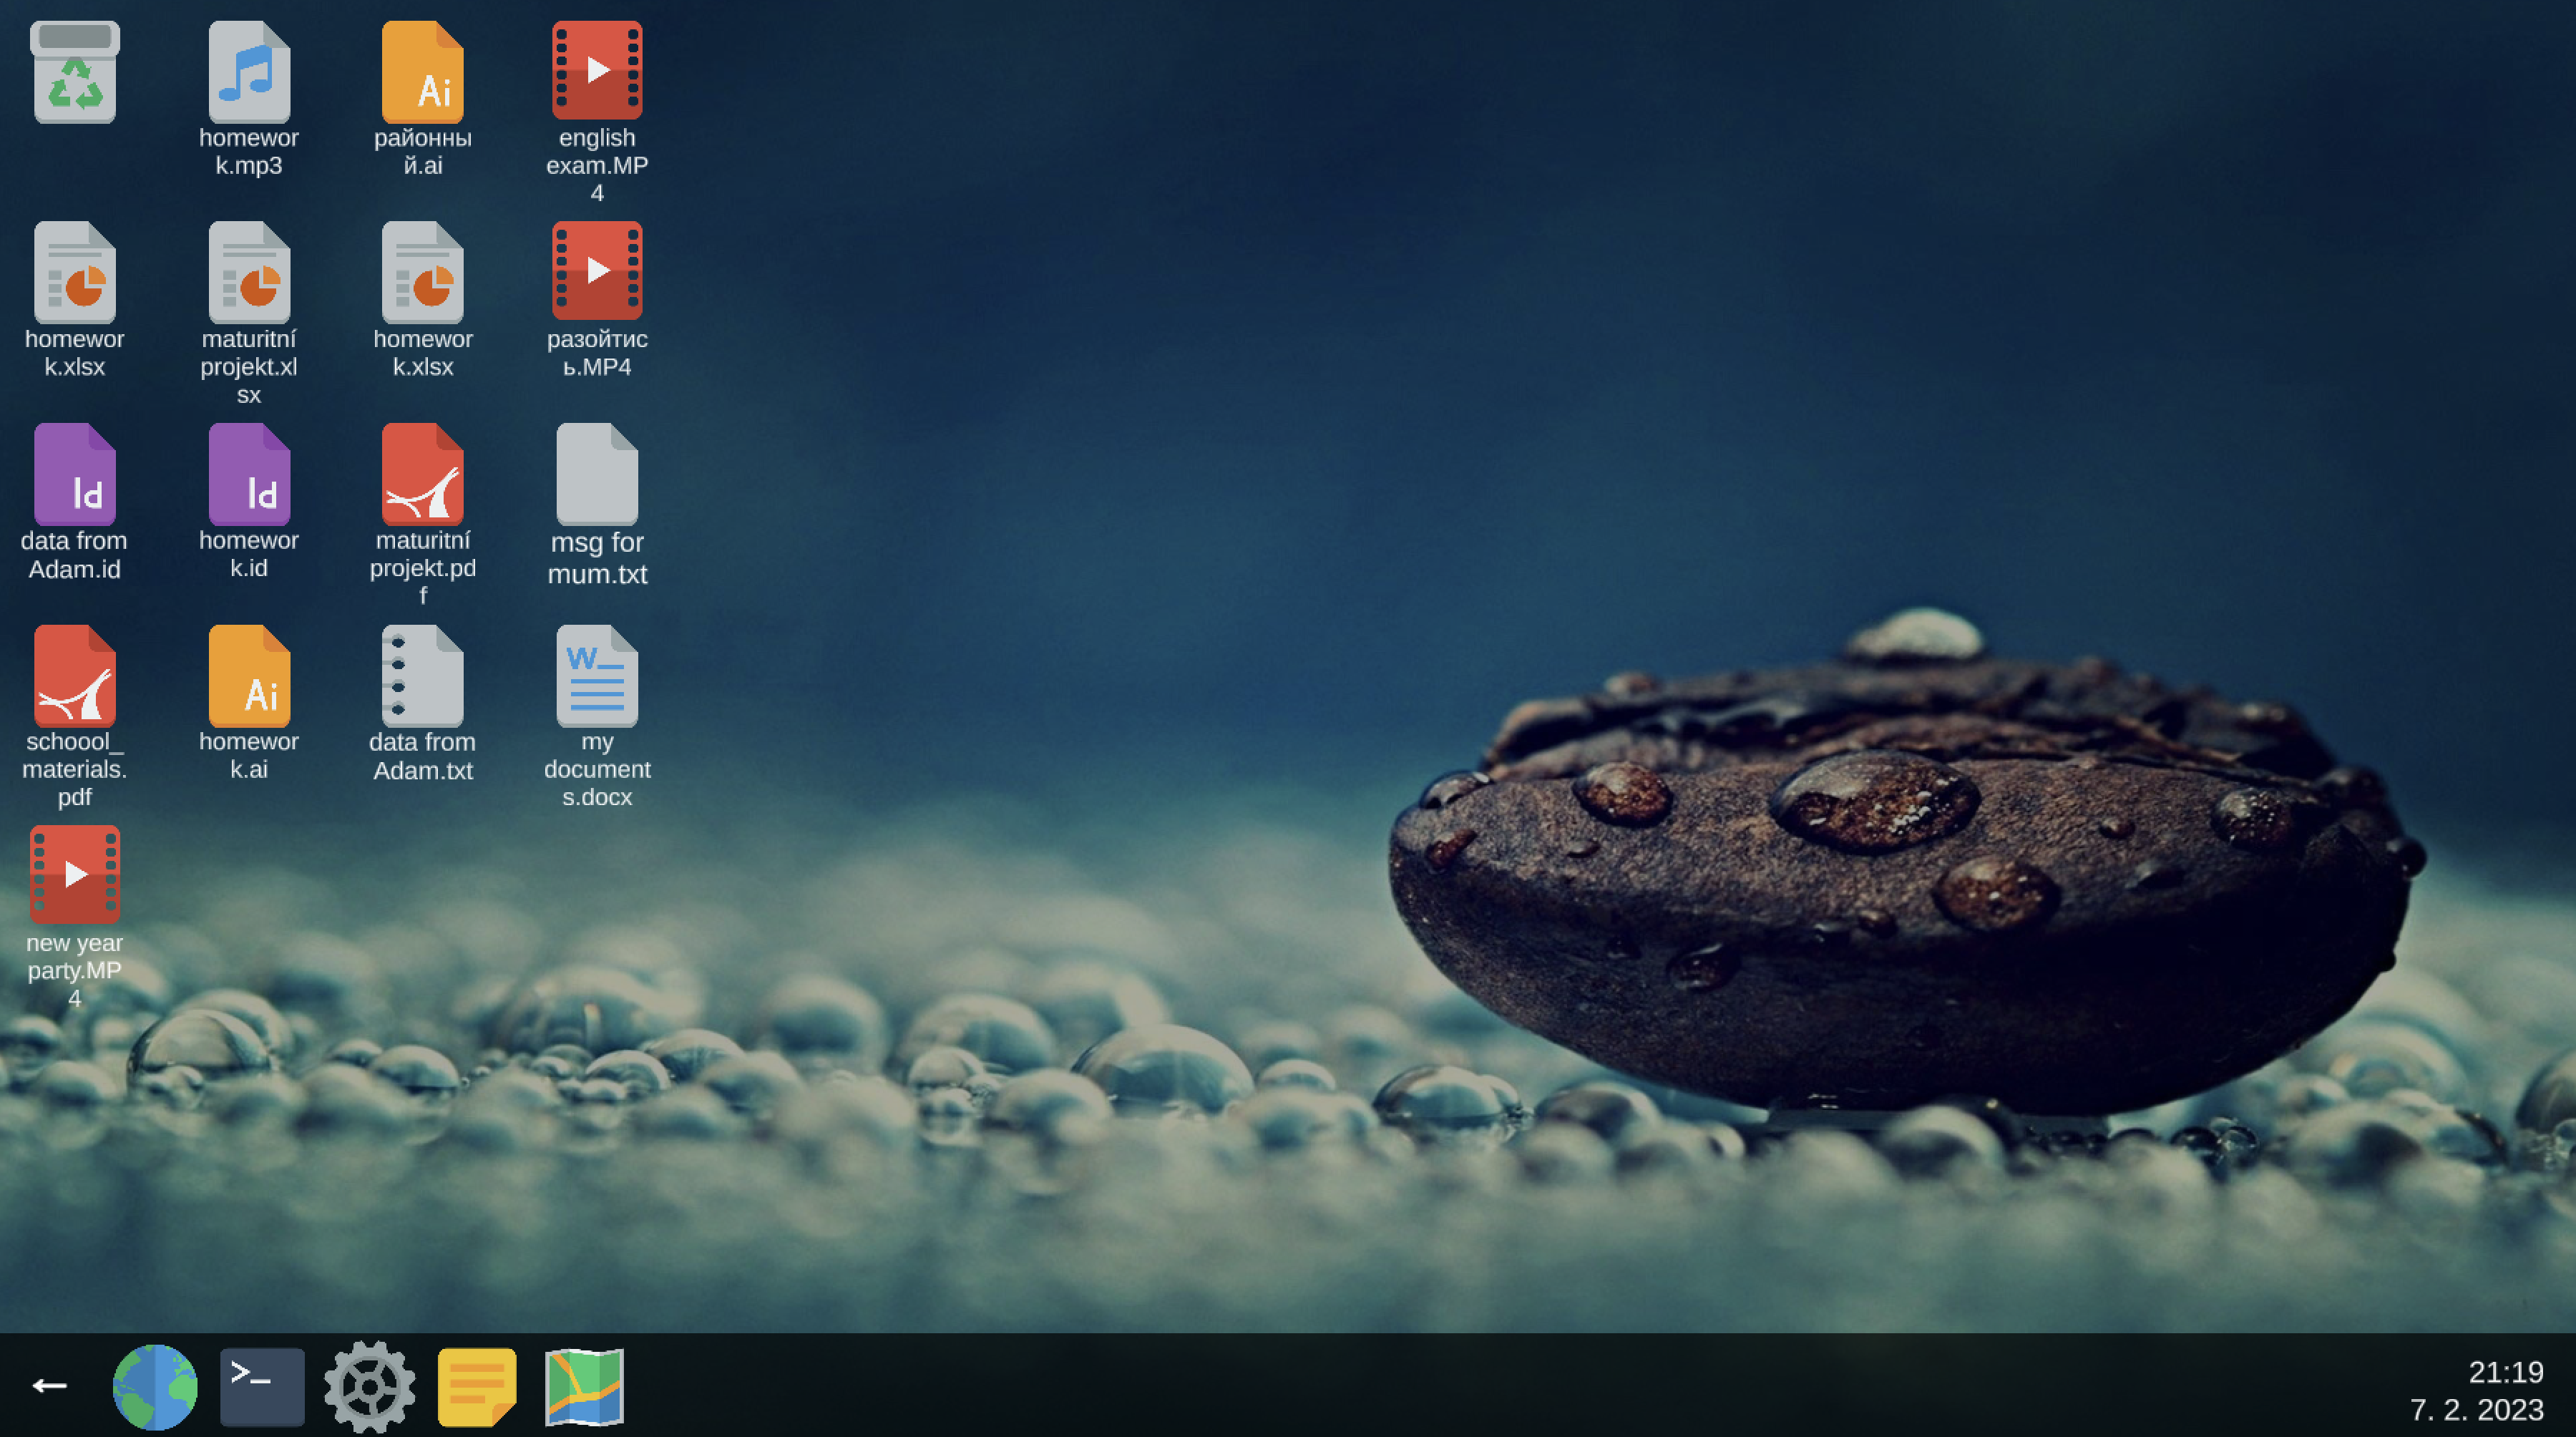
\includegraphics[width=\columnwidth]{pc0.png}
    \centering
    \caption{Ukázka grafického vzhledu počítačového rozhraní}
    \label{fig:pc0_img}
\end{figure}

\begin{figure}[ht]
    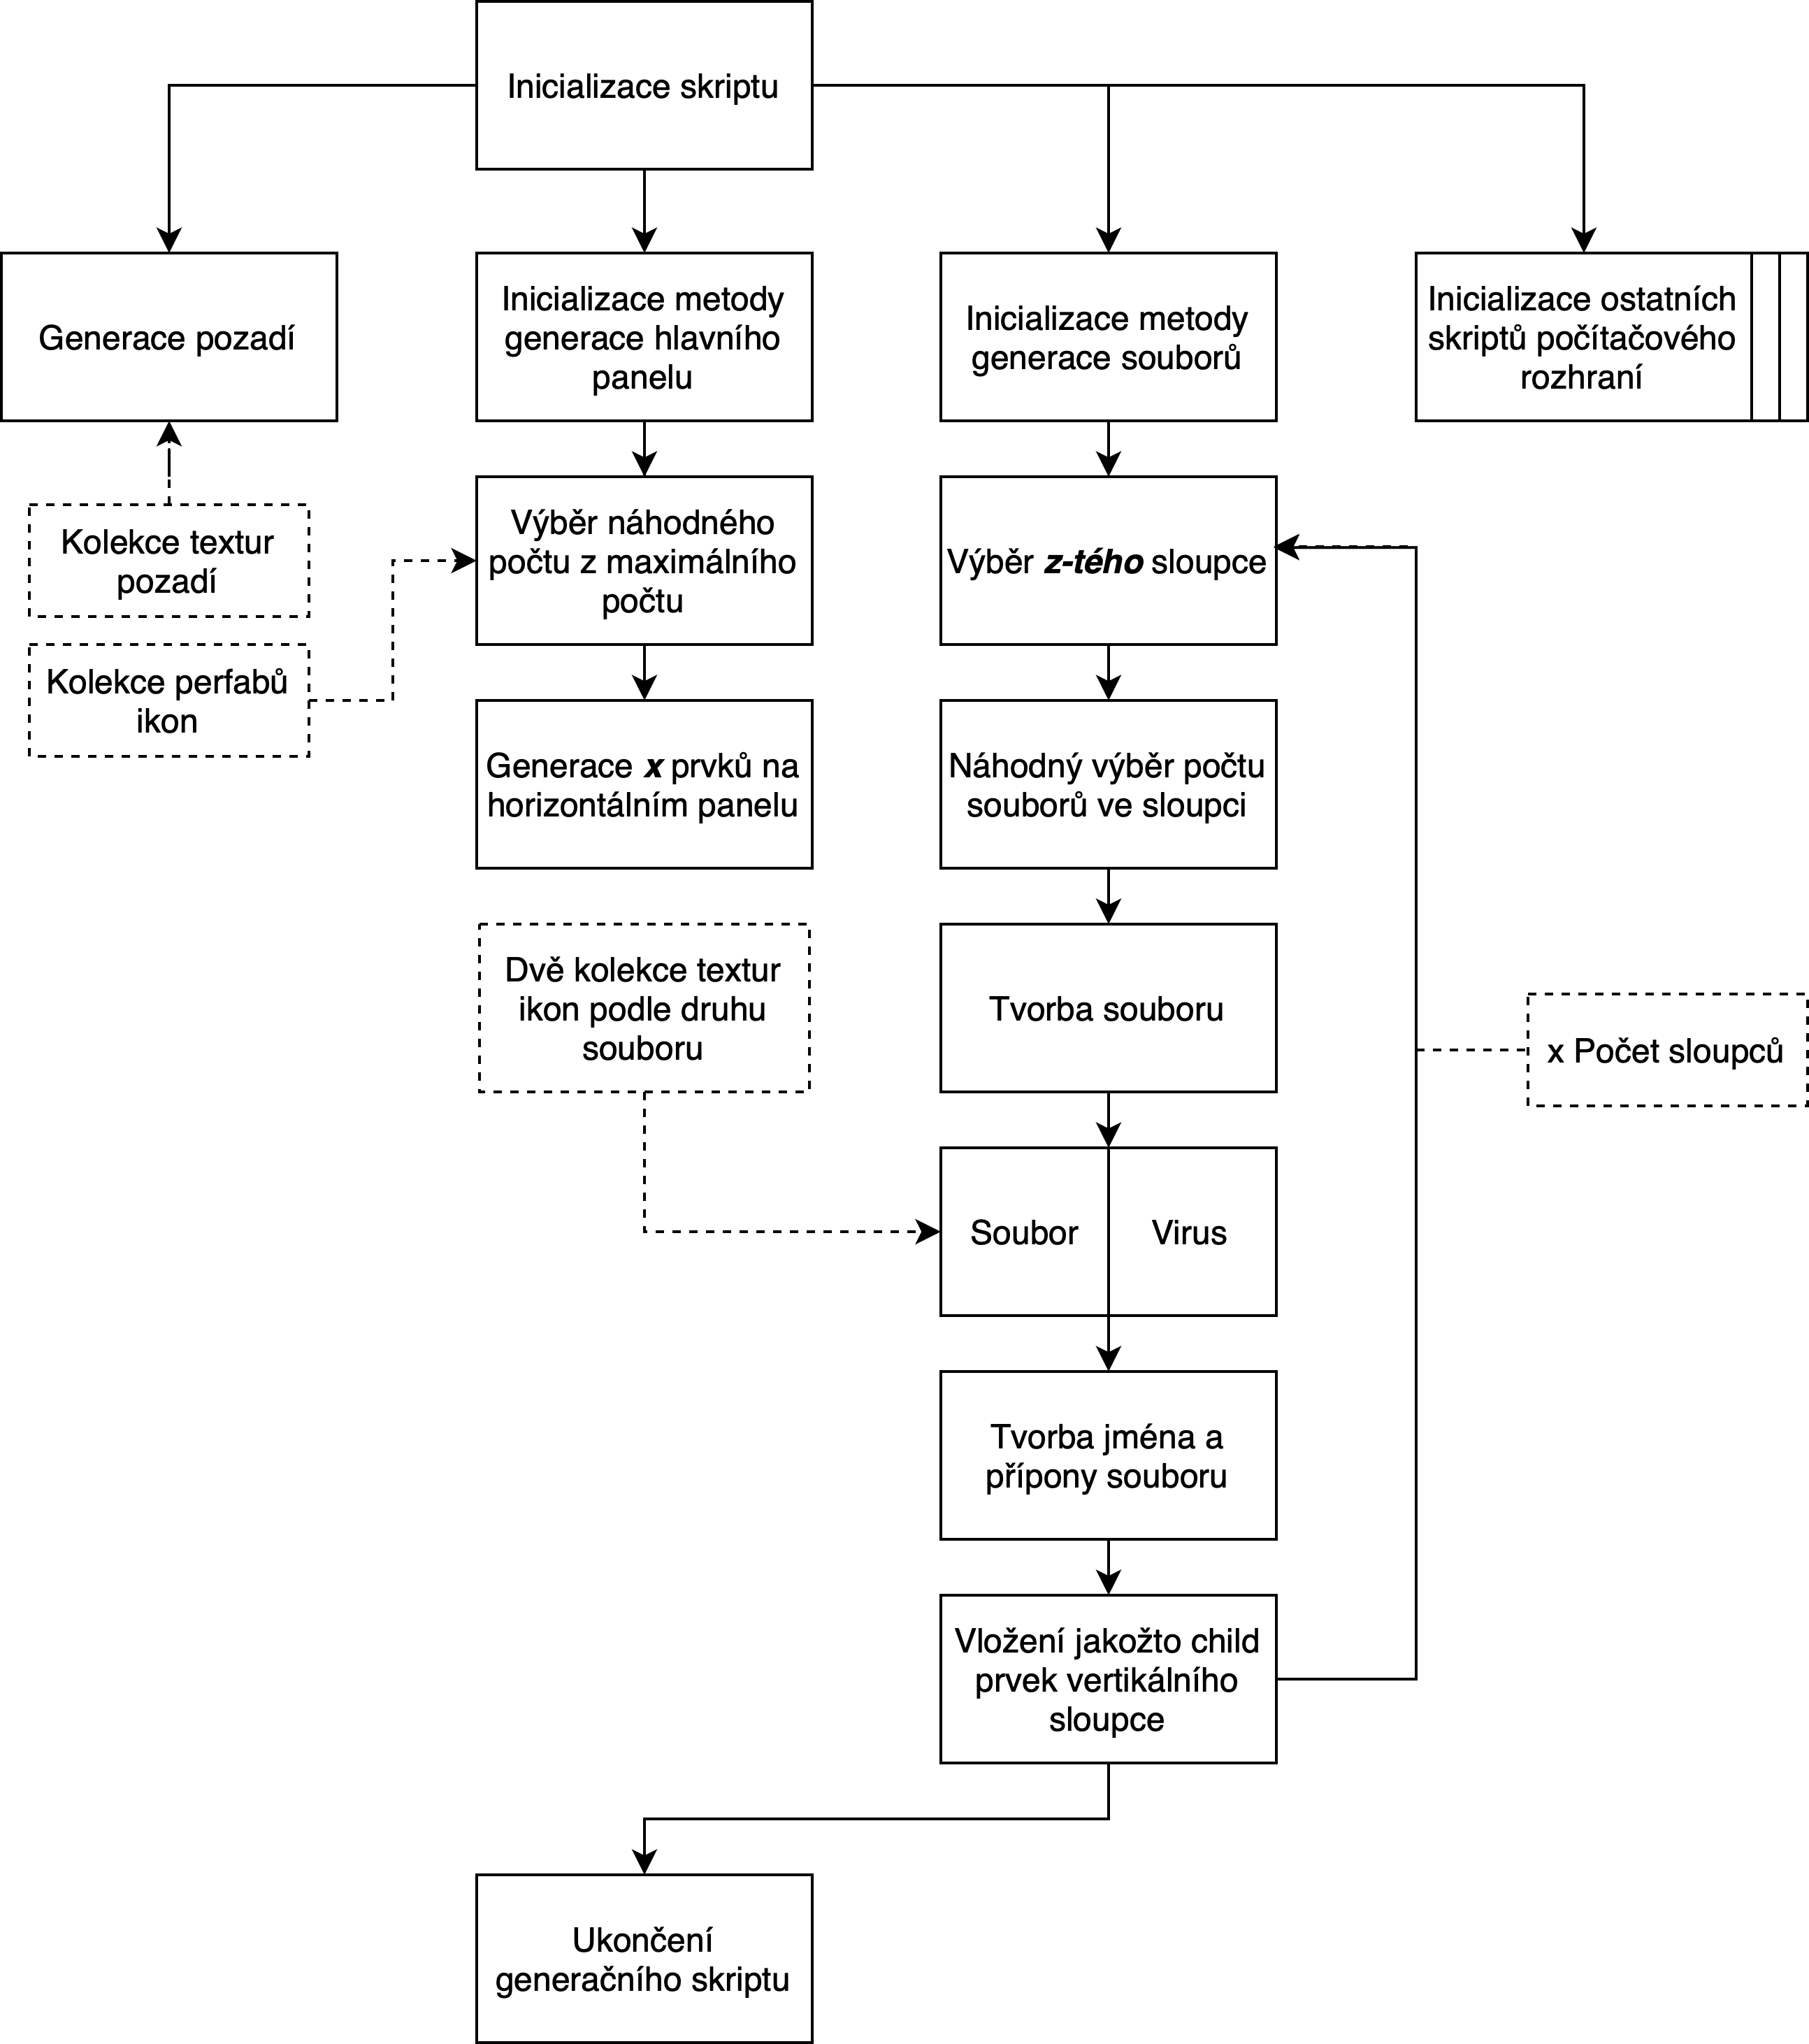
\includegraphics[width=\columnwidth]{generace_ui.png}
    \centering
    \caption{Znázornění generování grafického rozhraní}
    \label{fig:generace_ui_img}
\end{figure}

\subsection{Příkazový řádek a jeho modulární implementace}

V každé vytvořené počítačové stanici je na spodní hlavní liště umístěn příkazový řádek. V~této kapitole je popsáno jeho technické řešení a modulární implementace. Více informací o jeho využití je popsáno v kapitole \ref{sec:o_prikazovem_radku} níže.

Vytvořený simulovaný příkazový řádek pro hru obsahuje dva skripty, které slouží k~ovládání zobrazování komponent a zpracování příkazů.

První skript řídí zobrazování komponent, které jsou přítomny na canvasu, jako jsou například pole pro zadávání příkazů a výstup. Tento skript reaguje na uživatelské vstupy a přizpůsobuje zobrazované komponenty podle aktuálního stavu příkazového řádku.

Druhý skript, který je modulární, zpracovává příkazy a definuje výstup podle specifikací pro každý počítač v hře. Tento skript získává parsované příkazy, které jsou zadány hráčem na příkazovém řádku a na základě těchto příkazů definuje výstup, který je následně hráči zobrazen.

Důležitou vlastností druhého skriptu je jeho modulárnost, která umožňuje snadné přidávání nových příkazů a rozšíření funkcionality příkazového řádku. Tento skript může být upraven podle potřeb herního prostředí a umožňuje přidat nové příkazy a definovat výstupy pro každý z nich na základě unikátních parametrů každé počítačové stanice.

\section{Ovládání virtuálního počítače}
\label{sec:o_prikazovem_radku}

Výše zmíněný přikazový řádek je jedním z prvků, kterým lze počítač ovládat. Lze ho spustit kliknutím na ikonu na hlavním liště počítače. Hráč je částečně s jeho fungováním seznámen již v sekci výuky. V této sekci je popsána jeho interakce s uživatelem a následně několik dalších zůsobů, kterými může uživatel s virtuálním počítačem v aktuální verzi hry komunikovat.

Řádek simuluje pouze několik nejčastějších a nejjednoduších příkazů. Rozcestníkem pro tyto příkazy je stejně jako v opravdovém příkazovém řádku příkaz \textit{help}. Výstupem příkazu \textit{help} je seznam všech příkazů, které jsou momentálně dostupné. Patří mezi ně například: cd, dir, del, getmac, ipconfig, netstat, aj.

Dále počítačové rozhraní obsahuje generované soubory jejichž generace je popsána v~kapitole \ref{sec:generace_rozhrani}. Tyto soubory se skládají z ikony, názvu a přípony. Každý z těchto prvků může indikovat nebezpečný soubor. Je tak učiněno očividným způsobem.

\section[Řešení výukového scénáře]{Technické řešení výuky hráče}
\label{sec:vyuka_scenar_reseni}
Výuka hráče je tvořena několika scénami. Obzvláště v tomto scénáři bylo využito velké monožství prefabů z důvodu dodatečné optimalizace. 

V levé části každé scény se nachází textový popis, který je vložen v textovém boxu. Tento text je doplněn otázkami s interaktivními odpověďmi.

V pravé části se nachází 3D prostor zobrazující jedinou místnost s počítačovou stanicí. Je tak učiněno z důvodu minimalizace rozptylujících prvků. Tato stanice je stejně jako ostatní stanice ve hře interaktivní a hráč tedy má množnost vstoupit do počítačového rozhraní. Toto rozhraní je však lehce odlišné. Je značně omezeno z důvodu dodržení průběhu výuky. Některé části nejsou hráči dostupné, dostupné jsou pouze ty, které se v~danou chvíli týkají probíraného tématu.

\section{Postupy optimalizace}
\subsection{URP}
URP (Universal Render Pipeline) je vysokoúrovňový renderovací systém v Unity, který umožňuje vývojářům vytvářet graficky náročné hry s vysokým výkonem a škálovatelností. URP používá moderní technologie renderování, jako je například Deferred Rendering, které umožňují vytvářet sofistikované vizuální efekty a osvětlení. URP také podporuje funkce jako světelné sondy, post-processing a jednoduchou implementaci VR. URP je navržen tak, aby umožňoval vývojářům snadno optimalizovat výkon svých her. \cite{unity_urp}

Díky využití těchto jednoduše přístupných nastavení byla hra odladěna pro optimální výkon. Samozřejmě by se bylo možné optimalizací v tomto směru zabývat dále.

\subsection{Optimalizace skriptů}
Využití správných metod a privátních proměnných jsou důležité faktory pro optimalizaci výkonu skriptů v Unity. Když je použita funkce FixedUpdate namísto funkce Update pro aktualizaci fizikálního pohybu herních objektů, získává se stabilnější pohyb bez fluktuací.

Dále by měly být používány privátní proměnné místo veřejných proměnných, protože přístup k veřejným proměnným způsobuje značné zpomalení. Použití objektů jako parametrů funkcí také způsobuje zpomalení, proto by měly být použity proměnné. Navíc by mělo být minimalizováno použití funkcí Find() a GetComponent() v kódu, protože jsou to náročné operace. Místo toho by měl být uložen odkaz na herní objekt jako proměnná a mělo by být k němu přistupováno přímo. Dále by mělo být minimalizováno použití StartCoroutine() kvůli zpomalení a zvýšení náročnosti na paměť.

Výše uvedené optimalizační metody byly použity v projektu a jsou jedním z hlavních faktorů vedoucích ke zvýšení výkonu a především plynulosti celé hry.
\subsection{Occlusion culling}
Princip optimalizace za pomocí Occlusion culling v Unity spočívá v minimalizaci počtu objektů, které jsou renderovány v každém snímku, aby se zvýšila výkonnost a snížily nároky na grafickou kartu.

Occlusion culling využívá informace o viditelnosti, aby určil, které objekty jsou skryty za jinými objekty, a proto nejsou viditelné z pozice kamery. Pokud jsou tyto objekty skryty, nemusí být renderovány, což snižuje počet operací renderování v každém snímku.

Occlusion culling funguje tak, že se vytvoří prostorový graf scény, který reprezentuje vztahy mezi objekty a pozicí kamery. Poté se provede test viditelnosti, který pro každou kameru určí, které objekty jsou viditelné a které jsou skryté. Tyto informace se pak použijí ke generování listu viditelných objektů pro každou kameru.

V Unity se Occlusion culling provádí pomocí technologie Umbra, která umožňuje vytváření prostorových grafů scény a testování viditelnosti. Pro optimalizaci je důležité správně nastavit parametry Umbra, jako jsou velikost buněk, kvalita stínů a počet hierarchických úrovní.

V projektu byla nejprve vytvořena mapa a její prvky přetypovány na statické. Následně byla za pomocí skriptu spuštěna metoda StaticOclussionCulling.GenerateInBackground(), která vytvořila prostorový graf scény a provedla test viditelnosti. Výsledkem byl seznam viditelných objektů pro hlavní kameru, který byl uložen do souboru. Tento soubor byl následně načten do projektu a použit pro optimalizaci Occlusion cullingu.



\newpage

\chapter{Závěr}
Výsledným produktem je cílená beta verze projektu, která obsahuje všechny základní prvky, které jsou potřebné pro testování a další vývoj.

Sekce učení již podle předběžných testů úspěšně seznamuje hráče s probíranými tématy. Zároveň byl dodržen modulární postup řešení. Neměl by tedy být problém přidat další témata nebo upravit již existující.

Sekce náhodného scénáře dokresluje výše zmíněnou edukativní sekci. Zároveň je taktéž poměrně zajímavá ze svého technického hlediska, díky využité generaci prostředí.

Jedním z plánovaných prvků, ze kterých bylo bohužel potřeba v průběhu vývoje upustit, byla kompletní tvorba autorské grafiky. Nebylo tak učiněno z důvodu náročnosti, ale především s ohledem na časový rámec projektu. Do budoucna by však bylo vhodné vytvořit vlastní grafiku, která by mohla do jisté míry předefinovat celkový dojem z grafické stylizace.

V aktuální době je raná beta verze hry spustitelná na adrese \url{https://martas1293.itch.io/outside-the-net}.

Do budoucna je plánováno uzavřené testovaní hry. Toto testování bude mít za cíl získat zpětnou vazbu od hráčů, která bude sloužit k úpravám a vylepšení hry. Zároveň bude sloužit k ověření funkčnosti hry, identifikaci chyb a analýze výkonu. Dle přeběžných odhadů by se mělo testování zúčastnit několik málo desítek uživatelů.

\begin{flushleft}
\begin{thebibliography}{99}

\bibitem{isaca}
\textit{State of Cybersecurity 2022 Report: What’s the Current State of Cybersecurity?} [online]. Schaumburg, Illinois, USA: ISACA, 2022 [cit. 2023-03-22]. Dostupné z:~\url{https://www.isaca.org/go/state-of-cybersecurity-2022}

\bibitem{ita}
, \textit{ITU-D Study Group 2 a Telecommunication Development Bureau (BDT) Management Consultation Group. Global Cybersecurity Index 2020} [online]. 4. Ženeva, Švýcarsko: Mezinárodní telekomunikační unie, 2023 [cit. 2023-03-22]. ISBN 978-92-61-33921-0. Dostupné z: \url{https://www.itu.int/epublications/publication/D-STR-GCI.01-2021-HTM-E}

\bibitem{nukib}
\textit{Národní úřad pro kybernetickou a informační bezpečnost: Aktuality} [online]. Mučednická 1125/31, Brno, 616 00, Česko: Národní úřad pro kybernetickou a informační bezpečnost, 2023 [cit. 2023-03-20]. Dostupné z: \url{https://www.nukib.cz/cs/infoservis/aktuality/}

\bibitem{unity}
\textit{Unity Documentation: Docs and guides to work with the Unity ecosystem}  [online]. San Francisco, Kalifornie, USA: Unity Technologies, c2023 [cit. 2023-03-19]. \\Dostupné z: \href{https://docs.unity.com}{https://docs.unity.com}

\bibitem{unity_api}
\textit{Graphics API support} [online]. San Francisco, Kalifornie, USA: Unity Technologies, 2023 [cit. 2023-03-20]. Dostupné z: \href{https://docs.unity3d.com/Manual/GraphicsAPIs.html}{https://docs.unity3d.com/Manual/GraphicsAPIs.html}

\bibitem{unreal_engine}
\textit{Unreal Engine: The world’s most open and advanced real-time 3D creation tool} [online]. Cary, Severní Karolína, USA: Epic Games, c2004–2023 [cit. 2023-03-22]. Dostupné z: \url{https://www.unrealengine.com/en-US}

\bibitem{cryengine}
\textit{CryEngine: Achieve Your Vision} [online]. Frankfurt nad Mohanem, Německo: Crytek, c2023 [cit. 2023-03-22]. Dostupné z: \url{https://www.cryengine.com}

\bibitem{godot}
\textit{Godot: The game engine you've been waiting for.} [online]. -: Juan Linietsky, Ariel Manzur and contributors, c2007–2023 [cit. 2023-03-22]. Dostupné z: \url{https://godotengine.org}

\bibitem{rider}
\textit{JetBrains Rider 2022.3: Unity} [online]. Praha, Česko: JetBrains, c2000–2023 [cit. 2023-03-19]. Dostupné z: \href{https://www.jetbrains.com/help/rider/Unity.html}{https://www.jetbrains.com/help/rider/Unity.html}

\bibitem{riderflow}
\textit{RiderFlow for Unity: Scenery tool to build and manage your 3D space} [online]. Česko, Praha: JetBrains, c2000–2023 [cit. 2023-03-22]. Dostupné z: \url{https://www.jetbrains.com/riderflow/}

\bibitem{blender}
\textit{Blender 3.4 Reference Manual} [online]. Amsterdam, Nizozemsko: Blender Foundation, 2023 [cit. 2023-03-20]. Dostupné z: \href{https://docs.blender.org/manual/en/latest/}{https://docs.blender.org/manual/en/latest/}

\bibitem{unity_asset}
\textit{Simple Office Interiors - Cartoon assets} [online]. San Francisco, Kalifornie, USA: Unity Technologies, c2023 [cit. 2023-03-20]. Dostupné z: \href{https://assetstore.unity.com/packages/3d/props/interior/simple-office-interiors-cartoon-assets-38028}{https://assetstore.unity.com/packages/3d/props/interior/simple-office-interiors-cartoon-assets-38028}

\bibitem{enisa}
\textit{ARDAGNA, Claudio, Stephen CORBIAUX, Koen VAN IMPE a Andreas SFAKIANAKIS, LELLA, Ifigenei, Eleni TSEKMEZOGLOU, Rossen SVETOZAROV NAYDENOV, Cosmin CIOBANU, Apostolos MALATRAS a Marianthi THEOCHARIDOU, ed. ENISA Threat Landscape 2022.} 1. Iraklio, Řecko: European Union Agency for Cybersecurity (ENISA), 2022. ISBN 978-92-9204-588-3. \\Dostupné z: \href{https://www.enisa.europa.eu/publications/enisa-threat-landscape-2022}{https://www.enisa.europa.eu/publications/enisa-threat-landscape-2022}

\bibitem{unity_imput_system}
\textit{Input System} [online]. San Francisco, Kalifornie, USA: Unity Technologies, 2023 [cit. 2023-03-20]. Dostupné z: \href{https://docs.unity3d.com/Packages/com.unity.inputsystem@1.5/manual/index.html}{https://docs.unity3d.com/Packages/com.unity.inputsystem@1.5/manual/index.html}

\bibitem{unity_tmp}
\textit{TextMeshPro} [online]. San Francisco, Kalifornie, USA: Unity Technologies, 2023 [cit. 2023-03-20]. Dostupné z: \href{https://docs.unity3d.com/Manual/com.unity.textmeshpro.html}{https://docs.unity3d.com/Manual/com.unity.textmeshpro.html}

\bibitem{unity_scriptable_object}
\textit{ScriptableObject} [online]. San Francisco, Kalifornie, USA: Unity Technologies, 2023 [cit. 2023-03-20]. Dostupné z: \href{https://docs.unity3d.com/Manual/class-ScriptableObject.html}{https://docs.unity3d.com/Manual/class-ScriptableObject.html}

\bibitem{unity_baked_light}
\textit{Light Mode: Baked} [online]. San Francisco, Kalifornie, USA: Unity Technologies, 2023 [cit. 2023-03-20]. Dostupné z: \href{https://docs.unity3d.com/Manual/LightMode-Baked.html}{https://docs.unity3d.com/Manual/LightMode-Baked.html}

\bibitem{unity_build}
\textit{Build Settings} [online]. San Francisco, Kalifornie, USA: Unity Technologies, 2023 [cit. 2023-03-20]. Dostupné z: \href{https://docs.unity3d.com/Manual/BuildSettings.html}{https://docs.unity3d.com/Manual/BuildSettings.html}

\bibitem{unity_urp}
\textit{Universal Render Pipeline overview} [online]. San Francisco, Kalifornie, USA: Unity Technologies, 2023 [cit. 2023-03-20]. Dostupné z: \href{https://docs.unity3d.com/Packages/com.unity.render-pipelines.universal@16.0/manual/index.html}{https://docs.unity3d.com/Packages/com.unity.render-pipelines.universal@16.0/manual/index.html}

\end{thebibliography}
\end{flushleft}

\listoffigures

\vspace{0.5cm}
\textit{Veškeré užité obrázky jsou dílem autora práce.} \vspace{0.5cm}

\textit{Veškeré diagramy vložené fomrmou obrázku jsou dílem autora práce. Vytvořeny byly za pomocí bezplatného, volně dostupného open source softwaru Diagrams.net. Dostupné z: \url{https://app.diagrams.net}} \hangindent=0.7cm
% \listoftables

% \appendix

% \titleformat{\chapter}[block]{\scshape\bfseries\LARGE}{\thechapter}{10pt}{\vspace{0pt}}[\vspace{-22pt}] %% nastavení nadpisu u příloh

% \chapter*{Příloha}

% \chapter*{Zadání maturitního projektu z informatických předmětů}
\begin{tabular}{l l}
    Jméno a příjmení: & Martin Dobruský \\
    Pro školní rok: & 2022/2023 \\
    Třída: & 4. \\
	Obor: & Informační technologie 18-20-M/01 \\\\

    Téma práce: & Návrh a tvorba hry Outside The Net \\
    Vedoucí práce: & Mgr. Josef Horálek, Ph.D. \\
\end{tabular} \\\\

Způsob zpracování, cíle práce, pokyny k obsahu a rozsahu práce: \\
Cílem maturitního projektu je navrhnout a vytvořit videohru Outside The Net, jejímž cílem bude formou hry seznámit hráče s principy etického hackingu a zabezpečení výpočetních a komunikačních systémů. Hra bude 3D a bude hráči nabízet přímou interakci s infrastrukturou sítě. Ve hře budou obsaženy i principy hackingu netechnicky založené, například metoda Phishing. Hráč bude tedy seznámen s nejčastějšími pojmy v oboru zabezpečení výpočetní techniky a komunikačních systémů. Autor práce navrhne logické části hry Outside The Net vybere nejčastější bezpečností hrozby a způsob jejich začlenění do hry. V praktické části autor realizuje návrh Outside The Net za využití herního enginu Unity. Pilotním jazykem práce bude jazyk C\#, který bude využit s důrazem na standardy OOP. Pro tvorbu 3D assetů bude využit software Blender. \\\\
Stručný časový harmonogram (s daty a konkretizovanými úkoly): \\
Září – Říjen 2022 \\
\hspace{1cm}Návrh principů hry Outside The Net \\
Listopad – Prosinec 2022 \\
\hspace{1cm}Definování, a realizace dílčích částí hry Outside The Net \\
Prosinec – Únor 2022/2023 \\
\hspace{1cm}Komplexní implementace navrženého řešení \\
Únor – Březen 2023 \\
\hspace{1cm}Dokončení praktických řešení \\
Březen 2023 \\
\hspace{1cm}Finalizace textového znění maturitního projektu \\


\end{document}